\section{Hybrid 6-bit Floating-Point Computation}
\tableofcontents[currentsection]

\begin{frame}{Convolution Operation}
	\begin{figure}
		\centering
		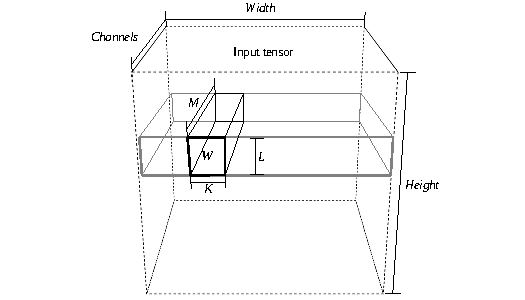
\includegraphics[width=0.5\textwidth]{../figures/convolution.pdf}
		\caption{\scriptsize Two dimensional convolution operation.}
	\end{figure}
	
	%\pause % Pause for the equation to appear after the image
	
	% Equation at the bottom
	{\scriptsize
		\[
Conv2D\left(W,b,h\right)_{i,j,o}=\sum_{k,l,m}^{K,L,M} h_{(i+k,j+l,m)} W_{(o,k,l,m)}+b_{o}
		\]
	}
\end{frame}

\begin{frame}{HW/SW Co-Design Framework}
	\begin{columns}[c] % The [T] option aligns the tops of the columns
		
		% Left column for the first image
		\begin{column}{0.5\textwidth}
			\begin{figure}
				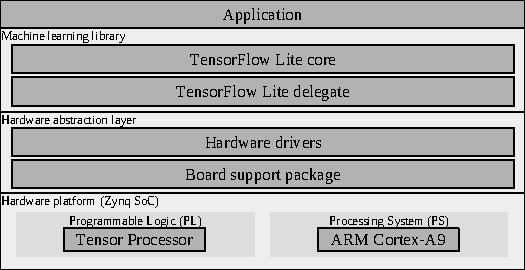
\includegraphics[width=\textwidth]{../chapters/cnn_accelerator/figures/sw_stack.pdf}
				\caption{\scriptsize High level embedded software architecture.}
			\end{figure}
		\end{column}
		
		% Right column for the second image
		\begin{column}{0.5\textwidth}
			\begin{figure}
				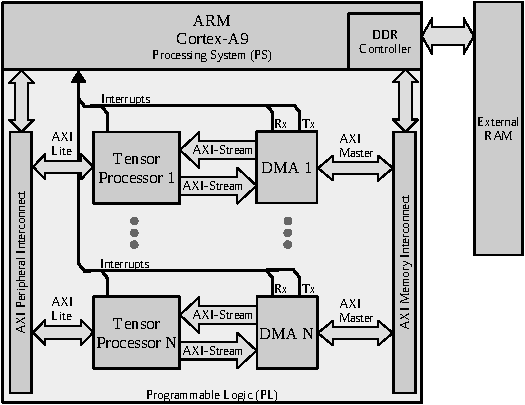
\includegraphics[width=0.8\textwidth]{../chapters/cnn_accelerator/figures/system_design.pdf} % Adjust the filename
				\caption{\scriptsize Base embedded system architecture.}
			\end{figure}
		\end{column}
		
	\end{columns}
\end{frame}

\begin{frame}{Tensor Processor}
	\begin{columns}[c] % The [T] option aligns the tops of the columns
		
		% Left column for the first image
		\begin{column}<1->{0.5\textwidth}
			\begin{figure}
				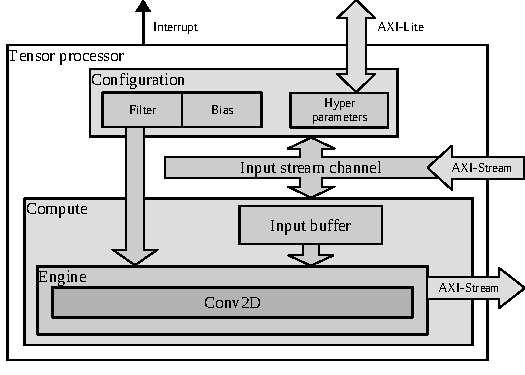
\includegraphics[width=0.7\textwidth]{../chapters/cnn_accelerator/figures/accelerator.pdf} % Adjust the filename
				\caption{\scriptsize High level architecture.}
			\end{figure}
		\end{column}
		
		% Right column for the second image
		\begin{column}<2->{0.5\textwidth}
			\begin{figure}
				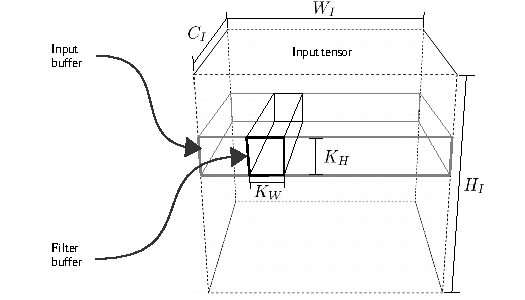
\includegraphics[width=0.9\textwidth]{../chapters/cnn_accelerator/figures/accelerator_buffers.pdf} % Adjust the filename
				\caption{\scriptsize On-chip memory buffers.}
			\end{figure}
		\end{column}
		
	\end{columns}
\end{frame}

\begin{frame}{On-Chip Memory}
	\begin{columns}[c] % The [T] option aligns the tops of the columns
		% Left column for equations
		\begin{column}{0.5\textwidth}
			\scriptsize
			\vspace{1mm}
			\begin{equation}
			TP_{M}=TP_B+V_{M}
			\end{equation}
			\vspace{1mm} 
			\begin{equation}
			TP_{B}=Input_{M}+Filter_{M}+Bias_{M}
			\end{equation}
			\vspace{1mm} 
			\begin{equation}
			Input_{M}=K_{H}W_{I}C_{I}BitSize_{I}
			\end{equation}
			\vspace{1mm} 
			\begin{equation}
			Filter_{M}=C_{I}K_{W}K_{H}C_{O}BitSize_{F}
			\end{equation}
			\vspace{1mm} 
			\begin{equation}
			Bias_{M}=C_{O}BitSize_{B}
			\end{equation}
			\vspace{1mm} 
			\begin{equation}
			C_{O}=\frac{TP_{M}-V_{M}-K_{H}W_{I}C_{I}BitSize_{I}}{C_{I}K_{W}K_{H}BitSize_{F}+BitSize_{B}}
			\end{equation}
		\end{column}
		
		% Right column for the image
		\begin{column}{0.5\textwidth}
			\begin{figure}
				\centering
				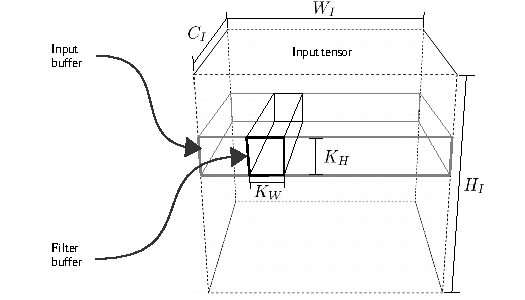
\includegraphics[width=0.9\textwidth]{../chapters/cnn_accelerator/figures/accelerator_buffers.pdf} % Adjust the filename
				\caption{\scriptsize On-chip memory buffers.}
			\end{figure}
		\end{column}
	\end{columns}
\end{frame}


\begin{frame}{Dot-Product with Hybrid Floating-Point 6-bit}
	\begin{columns}[c] % The [T] option aligns the tops of the columns
		
		% Left column for the first image
		\begin{column}<1->{0.5\textwidth}\centering
			\begin{figure}
				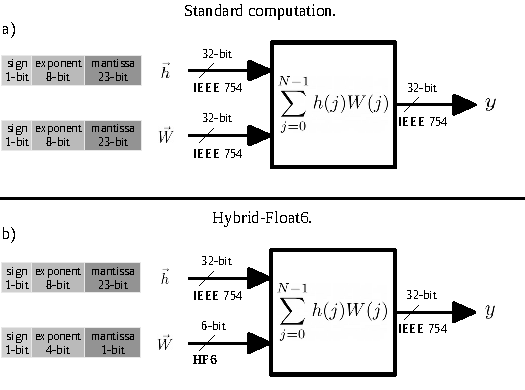
\includegraphics[width=0.75\textwidth]{../chapters/cnn_accelerator/figures/dot-product_unit.pdf} % Adjust the filename
				\caption{\scriptsize High level architecture.}
			\end{figure}
		\end{column}
		
		% Right column for the second image
		\begin{column}<2->{0.5\textwidth}
			\begin{figure}
				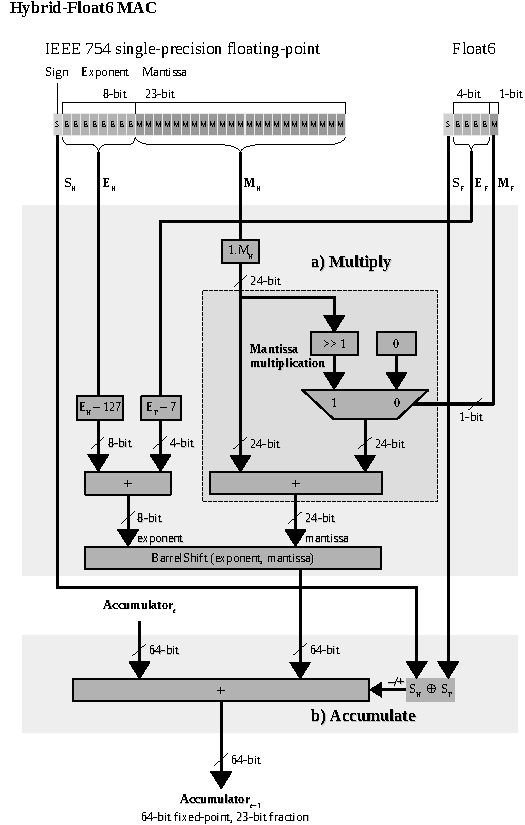
\includegraphics[width=0.5\textwidth]{../chapters/cnn_accelerator/figures/multiplier.pdf} % Adjust the filename
				\caption{\scriptsize On-chip memory buffers.}
			\end{figure}
		\scriptsize
		\[ L_{hf}=N+7 \]
		\end{column}
		
	\end{columns}
\end{frame}

\begin{frame}{Custom Floating-Point Quantization}
	\begin{figure}
		\centering
		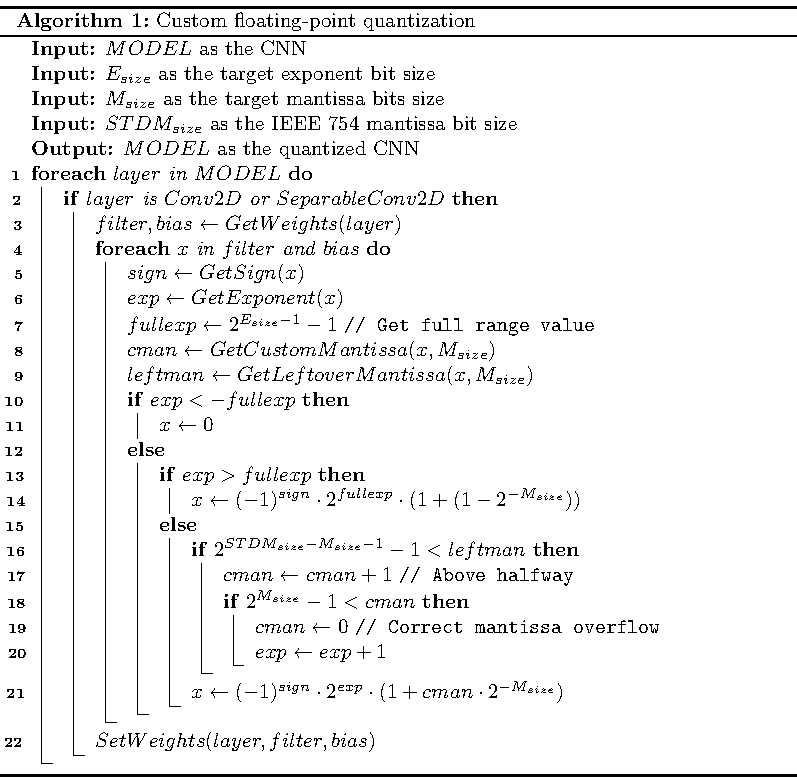
\includegraphics[width=0.6\columnwidth]{slides/algorithm_fp_2.pdf}
	\end{figure}
		
\end{frame}


\begin{frame}{Acceleration in Sensor Analytics (TinyML)}
	\begin{columns}[c] % The [T] option aligns the tops of the columns
		
		% Left column for the first image
		\begin{column}<1->{0.5\textwidth}\centering
			\begin{figure}
				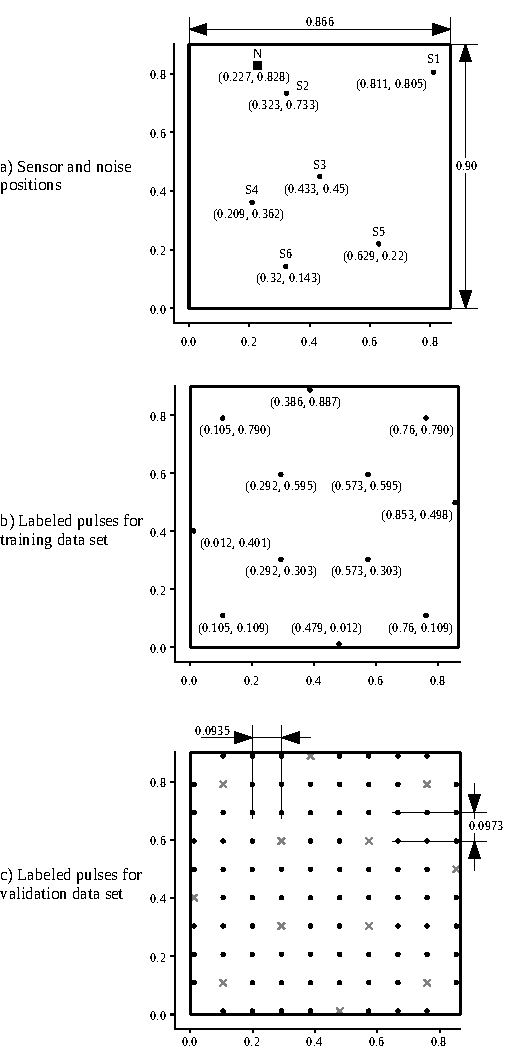
\includegraphics[width=0.5\textwidth]{../chapters/cnn_accelerator/figures/histograms/data_set.pdf} % Adjust the filename
				\caption{\scriptsize Structural health monitoring, all lengths are in metters (m).}
			\end{figure}
		\end{column}
		
		% Right column for the second image
		\begin{column}<2->{0.5\textwidth}
			\begin{figure}
				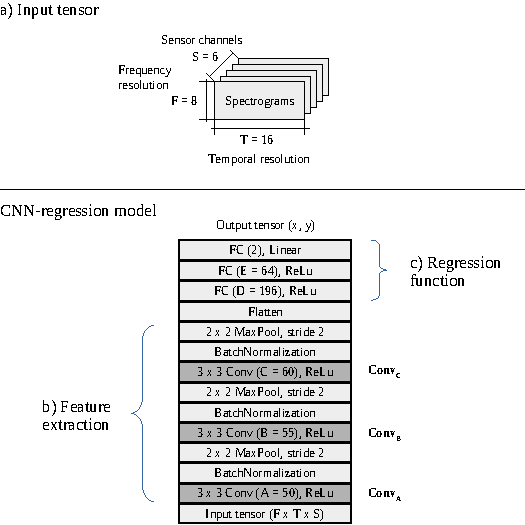
\includegraphics[width=0.75\textwidth]{../chapters/cnn_accelerator/figures/models.pdf} % Adjust the filename
				\caption{\scriptsize CNN-regression model for sensor analytics.}
			\end{figure}
		\end{column}
		
	\end{columns}
\end{frame}

\begin{frame}{Training}
	% Grid of images 2x2
	\begin{figure}
		\begin{minipage}[c]{0.48\linewidth}
			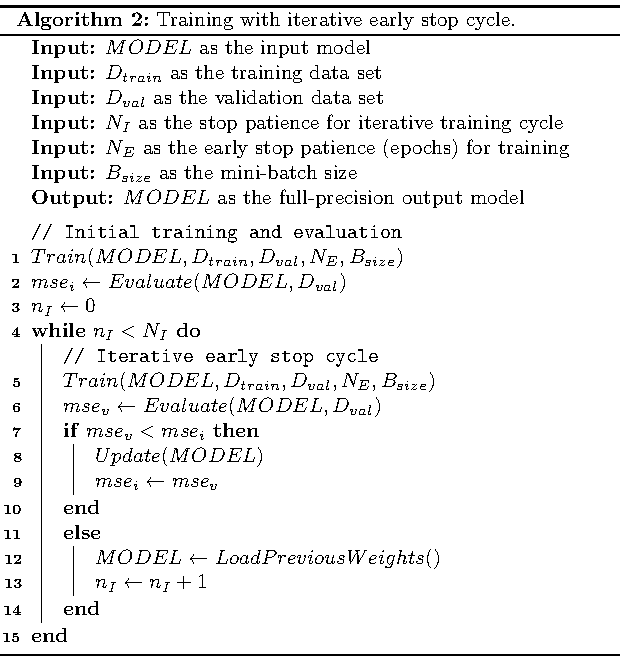
\includegraphics[width=0.6\linewidth]{slides/algorithm_early_stop_1.pdf} % Top left image
			\pause % Wait to reveal the next image
		\end{minipage}
		\hfill
		\begin{minipage}[c]{0.48\linewidth}
			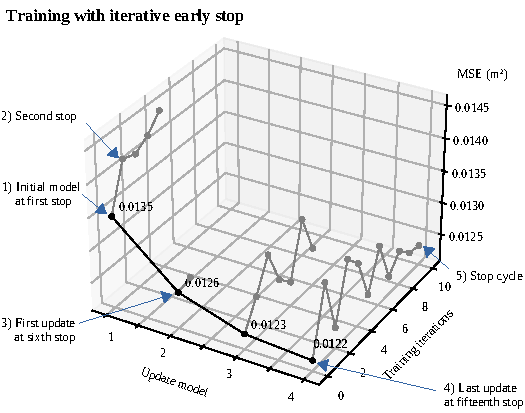
\includegraphics[width=0.6\linewidth]{slides/figures/training_iterative_early_stop.pdf} % Top right image
			\pause % Wait to reveal the next image
		\end{minipage}
		
		\vspace{0.5cm} % Vertical space between the rows of images
		
		\begin{minipage}[c]{0.48\linewidth}
			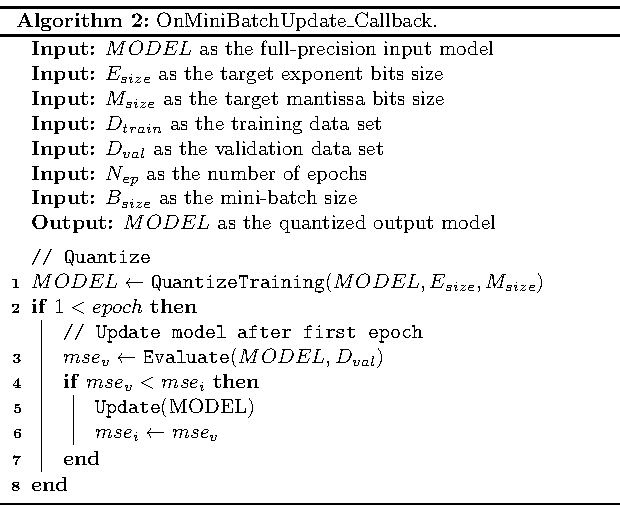
\includegraphics[width=0.6\linewidth]{slides/OnMiniBatchUpdate_2.pdf} % Bottom left image
			\pause % Wait to reveal the next image
		\end{minipage}
		\hfill
		\begin{minipage}[c]{0.48\linewidth}
			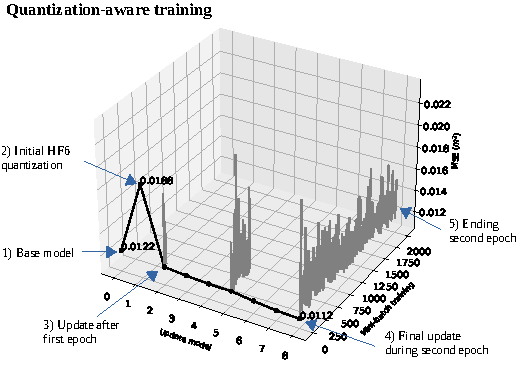
\includegraphics[width=0.6\linewidth]{slides/figures/QAT.pdf} % Bottom right image
		\end{minipage}
	\end{figure}
\end{frame}
